\documentclass[12pt,a4paper,oneside]{report}

% -----------------------------------------------------------------------------
% Packages and Formatting Setup
% -----------------------------------------------------------------------------
\usepackage[utf8]{inputenc}
\usepackage[margin=1in]{geometry}
\usepackage{times}
\usepackage{setspace}
\onehalfspacing

\usepackage{graphicx}
\usepackage{amsmath,amssymb}
\usepackage{booktabs}
\usepackage{tabularx}
\usepackage{multirow}
\usepackage{longtable}
\usepackage{enumitem}
\usepackage{fancyhdr}
\usepackage{titlesec}
\usepackage{xcolor}
\usepackage{listings}
\usepackage{tikz}
\usetikzlibrary{shapes.geometric, arrows, positioning}

\usepackage[colorlinks=true, linkcolor=blue!80!black, urlcolor=blue!70!black, citecolor=green!60!black]{hyperref}

% -----------------------------------------------------------------------------
% Code Listing Configuration
% -----------------------------------------------------------------------------
\definecolor{codegreen}{rgb}{0,0.6,0}
\definecolor{codegray}{rgb}{0.5,0.5,0.5}
\definecolor{codepurple}{rgb}{0.58,0,0.82}
\definecolor{backcolour}{rgb}{0.96,0.97,0.98}

\lstdefinestyle{customcode}{
    backgroundcolor=\color{backcolour},   
    commentstyle=\color{codegreen}\itshape,
    keywordstyle=\color{blue}\bfseries,
    numberstyle=\tiny\color{codegray},
    stringstyle=\color{codepurple},
    basicstyle=\ttfamily\footnotesize,
    breakatwhitespace=false,         
    breaklines=true,                 
    captionpos=b,                    
    keepspaces=true,                 
    numbers=left,                    
    numbersep=7pt,                  
    showspaces=false,                
    showstringspaces=false,
    showtabs=false,                  
    tabsize=2,
    frame=single,
    rulecolor=\color{black!20}
}
\lstset{style=customcode}

% -----------------------------------------------------------------------------
% Header & Footer Styling
% -----------------------------------------------------------------------------
\pagestyle{fancy}
\fancyhf{}
\fancyhead[L]{\small\nouppercase{\leftmark}}
\fancyhead[R]{\small Project KEYSTONE | Zidio Development}
\fancyfoot[C]{\thepage}
\renewcommand{\headrulewidth}{0.5pt}
\renewcommand{\footrulewidth}{0.5pt}

% Title formats
\titleformat{\chapter}[display]
  {\normalfont\huge\bfseries\color{blue!70!black}}
  {\chaptertitlename\ \thechapter}{14pt}{\Huge}
\titlespacing*{\chapter}{0pt}{0pt}{20pt}

% -----------------------------------------------------------------------------
% Document Body
% -----------------------------------------------------------------------------
\begin{document}

% =============================================================================
% Title Page
% =============================================================================
\begin{titlepage}
    \centering
    \vspace*{0.5cm}
    
    {\Huge\bfseries Project KEYSTONE\par}
    \vspace{0.4cm}
    {\Large\bfseries Enterprise Field Service Management (FSM) Platform\par}
    \vspace{0.2cm}
    {\large Full-Stack Architecture, Cloud-Native Containerization, and Continuous Deployment\par}
    
    \vspace{1.5cm}
    \rule{\linewidth}{1.5pt}\par
    \vspace{0.5cm}
    {\large\itshape A Technical Project Report submitted in partial fulfillment of the requirements for the Software Engineering Internship at\par}
    \vspace{0.5cm}
    {\LARGE\bfseries Zidio Development\par}
    \vspace{0.5cm}
    \rule{\linewidth}{1.5pt}\par
    
    \vspace{2cm}
    
    \begin{minipage}{0.48\textwidth}
        \begin{flushleft} \large
            \textbf{Submitted by:}\\
            \textbf{Yash Marathe}\\
            Software Engineering Intern\\
            GitHub: \href{https://github.com/Yash-Marathe91}{@Yash-Marathe91}
        \end{flushleft}
    \end{minipage}
    \hfill
    \begin{minipage}{0.48\textwidth}
        \begin{flushright} \large
            \textbf{Host Organization:}\\
            \textbf{Zidio Development}\\
            Internship Program 2026\\
            Track: Full-Stack Web Development
        \end{flushright}
    \end{minipage}

    \vfill
    {\large\bfseries October 2026}\par
\end{titlepage}

% =============================================================================
% Certificate / Declaration
% =============================================================================
\newpage
\chapter*{Candidate's Declaration}
\addcontentsline{toc}{chapter}{Candidate's Declaration}

I hereby declare that the work presented in this internship project report titled \textbf{"Project KEYSTONE: Enterprise Field Service Management (FSM) Platform"} is an authentic record of the development, engineering, and deployment work carried out by me during my internship tenure at \textbf{Zidio Development}.

The software architecture, database schemata, backend REST APIs, frontend user interfaces, and automated cloud deployment pipelines documented herein represent original engineering contributions, implemented with adherence to industry-standard software quality benchmarks and security frameworks.

\vspace{2.5cm}

\noindent
\begin{tabular}{@{}p{0.5\textwidth}p{0.5\textwidth}@{}}
\textbf{Date:} October 04, 2026 & \textbf{Yash Marathe} \\
\textbf{Place:} India & Software Engineering Intern, Zidio Development \\
\end{tabular}

% =============================================================================
% Acknowledgement
% =============================================================================
\newpage
\chapter*{Acknowledgements}
\addcontentsline{toc}{chapter}{Acknowledgements}

I express my deepest gratitude to the technical mentors and leadership team at \textbf{Zidio Development} for providing me with this opportunity to design and engineer an enterprise-grade solution during my internship. Their guidance on distributed micro-architectures, modern cloud infrastructure, and rigorous engineering practices was invaluable.

I would also like to thank the open-source engineering community whose contributions to Spring Boot, React, Vite, and containerization ecosystems made the accelerated development and robust deployment of Project KEYSTONE possible.

\vspace{1.5cm}
\noindent\textbf{Yash Marathe}

% =============================================================================
% Abstract
% =============================================================================
\newpage
\chapter*{Executive Summary}
\addcontentsline{toc}{chapter}{Executive Summary}

Field Service Management (FSM) represents a critical operational pillar for modern logistics, telecommunications, equipment maintenance, and facility management organizations. Traditional field operations frequently suffer from disparate operational tracking, manual scheduling bottlenecks, lack of real-time inventory visibility, and fragile synchronization between customer dispatch and field technician execution.

\textbf{Project KEYSTONE} is an enterprise-class, full-stack, cloud-native Field Service Management platform engineered to address these operational challenges. Built on a modular distributed architecture, KEYSTONE encompasses:
\begin{enumerate}[label=(\roman*)]
    \item \textbf{A High-Performance Backend}: Developed using \textbf{Spring Boot 3.4} and \textbf{Java 21 LTS}, featuring Spring Data JPA (Hibernate 6), Spring Security with stateless JSON Web Token (JWT) role-based access control (RBAC), HikariCP connection pooling, and Flyway migration versioning.
    \item \textbf{A Relational Cloud Database}: Hosted on \textbf{PostgreSQL 16} via \textbf{Supabase} in the Singapore (\texttt{ap-southeast-1}) AWS region, enforcing referential integrity across 8 normalized tables governing users, customers, dispatch sites, inventory parts, work orders, part consumption, and labor time tracking.
    \item \textbf{A Dynamic Single-Page Application (SPA)}: Built using \textbf{React 18/19}, \textbf{TypeScript}, \textbf{Vite}, and modern responsive styling, implementing end-to-end type safety, optimistic state management, interactive dispatch scheduling, and role-tailored dashboards.
    \item \textbf{Production DevOps \& Cloud Deployment}: Packaged via a multi-stage Docker build utilizing an Ubuntu Jammy LTS (\texttt{eclipse-temurin:21-jre-jammy}) glibc runtime deployed on \textbf{Render} Web Services, paired with an edge-replicated \textbf{Vercel} frontend deployment.
\end{enumerate}

This technical report comprehensively documents the end-to-end design, architectural specifications, database models, security implementations, cloud networking challenges (including IPv4/IPv6 compatibility and TLS 1.3 handshake resolution), and deployment outcomes of Project KEYSTONE.

% =============================================================================
% Tables of Contents, Figures, Tables
% =============================================================================
\newpage
\tableofcontents
\listoffigures
\listoftables

% =============================================================================
% Chapter 1: Introduction
% =============================================================================
\newpage
\chapter{Introduction}

\section{Background and Motivation}
In modern industrial, telecommunication, and enterprise service domains, customer satisfaction and operational efficiency depend fundamentally on the precision and velocity of field operations. Dispersed field technicians must receive timely dispatch requests, locate customer operational sites, review diagnostic histories, consume inventory parts, and log billable labor hours without friction. 

Legacy field management paradigms typically rely on fragmented legacy software, paper work orders, or manual spreadsheets. This fragmentation precipitates:
\begin{itemize}
    \item Severe communication latency between dispatchers and field technicians.
    \item Inaccurate inventory bookkeeping, leading to part shortages during critical maintenance visits.
    \item Inadequate auditability regarding actual on-site technician hours versus billed invoices.
    \item Lack of self-service visibility for commercial customers seeking updates on active service requests.
\end{itemize}

\section{Project Objectives}
Project KEYSTONE was conceived and engineered to establish a unified, secure, and resilient platform that centralizes the complete lifecycle of field operations. The core objectives are:
\begin{enumerate}
    \item \textbf{Role-Based Orchestration}: Provide distinct, fine-grained access control boundaries for Administrators, Dispatchers, Field Technicians, and Commercial Customers.
    \item \textbf{End-to-End Work Order Lifecycle}: Enable real-time creation, assignment, status tracking (\texttt{OPEN} $\rightarrow$ \texttt{ASSIGNED} $\rightarrow$ \texttt{IN\_PROGRESS} $\rightarrow$ \texttt{COMPLETED} $\rightarrow$ \texttt{CANCELLED}), and priority dispatching (\texttt{LOW}, \texttt{MEDIUM}, \texttt{HIGH}, \texttt{URGENT}).
    \item \textbf{Inventory Tracking}: Enforce automatic stock balance validation, part consumption logging against work orders, and low-stock alerting based on predefined threshold triggers.
    \item \textbf{Labor Logging \& Auditing}: Capture granular technician time logs tied to specific work order IDs, facilitating accurate labor calculations and audit compliance.
    \item \textbf{Cloud-Native Resilience}: Ensure high availability, container portability, and secure encrypted communication across distributed cloud hosting tiers (Render, Supabase, Vercel).
\end{enumerate}

\section{Project Scope and Deliverables}
The project delivers a fully functional, publicly deployed software ecosystem:
\begin{itemize}
    \item \textbf{Version Control Repository}: Maintained under Git and hosted at GitHub: \url{https://github.com/Yash-Marathe91/Field_Service_Management_Platform}.
    \item \textbf{Live RESTful Backend API}: Containerized and running on Render Web Services at: \url{https://field-service-management-platform-p2rj.onrender.com}.
    \item \textbf{Interactive Interactive API Documentation}: Built-in Swagger UI and OpenAPI 3.0 endpoints accessible at \texttt{/swagger-ui.html}.
    \item \textbf{Client SPA Application}: Hosted on Vercel delivering responsive desktop and mobile field interfaces.
    \item \textbf{Automated Database Initialization}: Comprehensive idempotent DDL and DML migration scripts provisioned in Supabase PostgreSQL.
\end{itemize}

% =============================================================================
% Chapter 2: System Architecture & Requirements
% =============================================================================
\newpage
\chapter{System Architecture \& Requirements}

\section{Functional Requirements}
The functional scope of Project KEYSTONE is structured around core business modules:

\begin{table}[htbp]
    \centering
    \caption{Functional Requirements Breakdown by Module}
    \label{tab:functional_reqs}
    \begin{tabularx}{\textwidth}{lXl}
        \toprule
        \textbf{Module} & \textbf{Key Functional Capabilities} & \textbf{Target Roles} \\
        \midrule
        \textbf{Authentication} & User registration, JWT-based login, token validation, secure password hashing (BCrypt). & All Users \\
        \textbf{Customer Mgmt} & CRUD operations for commercial accounts, contact records, multiple associated job sites. & Admin, Dispatcher \\
        \textbf{Site Management} & GPS coordinates (latitude/longitude), address mapping, customer binding. & Admin, Dispatcher \\
        \textbf{Work Orders} & Full lifecycle state machine, priority assignment, technician assignment, filtering, pagination. & Admin, Dispatcher, Tech \\
        \textbf{Inventory Mgmt} & Part cataloging, SKU tracking, stock level monitoring, real-time consumption deduction. & Admin, Dispatcher, Tech \\
        \textbf{Labor Logging} & Granular technician duration logs (minutes), descriptive notes, work order associations. & Technician, Admin \\
        \textbf{Analytics} & Aggregated KPI metrics: active work orders, customer count, technician utilization, stock alerts. & Admin, Dispatcher \\
        \bottomrule
    \end{tabularx}
\end{table}

\section{Non-Functional Requirements}
\begin{itemize}
    \item \textbf{Security \& Confidentiality}: All passwords hashed using BCrypt. Stateless JWT tokens signed using SHA-256 HMAC keys. Zero plain-text credential persistence. Cross-Origin Resource Sharing (CORS) restricted to verified frontend domains.
    \item \textbf{Performance \& Scalability}: Sub-100ms API response time for cached read queries. HikariCP connection pooling configured with aggressive idle/lifetime recycling.
    \item \textbf{Reliability \& Data Integrity}: Complete ACID compliance enforced via PostgreSQL foreign keys, unique indexes, and cascade restrictions.
    \item \textbf{Cloud Portability}: Complete isolation via Open Container Initiative (OCI) multi-stage Docker packaging, eliminating host-dependent environmental inconsistencies.
\end{itemize}

\section{System Architecture Diagram}
The architecture follows a decoupled, three-tier cloud-native model as illustrated below:

\begin{figure}[htbp]
    \centering
    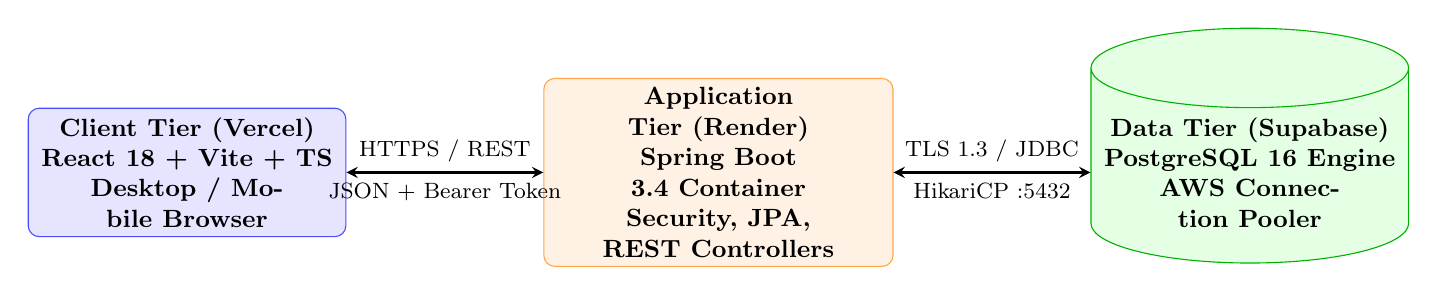
\begin{tikzpicture}[node distance=1.8cm, auto, >=stealth,
        client/.style={rectangle, draw=blue!70, fill=blue!10, rounded corners, text width=3.8cm, text centered, minimum height=1.3cm, font=\small\bfseries},
        cloud/.style={rectangle, draw=orange!70, fill=orange!10, rounded corners, text width=4.2cm, text centered, minimum height=1.5cm, font=\small\bfseries},
        db/.style={cylinder, draw=green!70!black, fill=green!10, shape border rotate=90, aspect=0.25, text width=3.8cm, text centered, minimum height=1.6cm, font=\small\bfseries}
    ]
        % Nodes
        \node [client] (fe) {Client Tier (Vercel)\\React 18 + Vite + TS\\Desktop / Mobile Browser};
        \node [cloud, right=2.5cm of fe] (be) {Application Tier (Render)\\Spring Boot 3.4 Container\\Security, JPA, REST Controllers};
        \node [db, right=2.5cm of be] (db) {Data Tier (Supabase)\\PostgreSQL 16 Engine\\AWS Connection Pooler};

        % Connectors
        \draw[<->, thick] (fe) -- node[above, font=\footnotesize] {HTTPS / REST} node[below, font=\footnotesize] {JSON + Bearer Token} (be);
        \draw[<->, thick] (be) -- node[above, font=\footnotesize] {TLS 1.3 / JDBC} node[below, font=\footnotesize] {HikariCP :5432} (db);
    \end{tikzpicture}
    \caption{Three-Tier Cloud-Native Architecture of Project KEYSTONE}
    \label{fig:architecture}
\end{figure}

% =============================================================================
% Chapter 3: Database Design & Schema Modeling
% =============================================================================
\newpage
\chapter{Database Design \& Schema Modeling}

\section{Entity-Relationship (ER) Overview}
The relational database design was architected to eliminate data redundancy while providing comprehensive referential integrity and performance indexing. The physical schema consists of seven core application tables plus an automated schema migration history table.

\section{Database Tables Specification}
The technical specifications of the core tables are outlined below:

\begin{table}[htbp]
    \centering
    \small
    \caption{Relational Database Schema Table Catalog}
    \label{tab:db_tables}
    \begin{tabularx}{\textwidth}{lp{4cm}X}
        \toprule
        \textbf{Table Name} & \textbf{Primary Key} & \textbf{Foreign Keys \& Constraints} \\
        \midrule
        \texttt{users} & \texttt{id} (BIGSERIAL) & \texttt{email} (UNIQUE, NOT NULL), \texttt{role} (CHECK IN ADMIN, DISPATCHER, TECHNICIAN, CUSTOMER) \\
        \texttt{customers} & \texttt{id} (BIGSERIAL) & \texttt{company\_name} (NOT NULL), \texttt{email} (VARCHAR) \\
        \texttt{sites} & \texttt{id} (BIGSERIAL) & \texttt{customer\_id} $\rightarrow$ \texttt{customers(id)} ON DELETE CASCADE \\
        \texttt{parts} & \texttt{id} (BIGSERIAL) & \texttt{part\_number} (UNIQUE, NOT NULL), \texttt{quantity\_on\_hand} ($\ge 0$) \\
        \texttt{work\_orders} & \texttt{id} (BIGSERIAL) & \texttt{work\_order\_number} (UNIQUE), \texttt{customer\_id} $\rightarrow$ \texttt{customers(id)}, \texttt{site\_id} $\rightarrow$ \texttt{sites(id)}, \texttt{assigned\_tech\_id} $\rightarrow$ \texttt{users(id)} \\
        \texttt{part\_usage} & \texttt{id} (BIGSERIAL) & \texttt{work\_order\_id} $\rightarrow$ \texttt{work\_orders(id)}, \texttt{part\_id} $\rightarrow$ \texttt{parts(id)} \\
        \texttt{time\_logs} & \texttt{id} (BIGSERIAL) & \texttt{work\_order\_id} $\rightarrow$ \texttt{work\_orders(id)}, \texttt{technician\_id} $\rightarrow$ \texttt{users(id)} \\
        \bottomrule
    \end{tabularx}
\end{table}

\section{Schema Constraints, Indexes, and Cascades}
To guarantee transactional performance and data consistency, specific database indexes and constraint triggers were engineered:
\begin{enumerate}
    \item \textbf{Unique Business Keys}: Work orders automatically generate an alphanumeric identifier (e.g., \texttt{WO-1001}) backed by a unique B-Tree index.
    \item \textbf{Foreign Key Indexing}: All relational join columns (\texttt{customer\_id}, \texttt{site\_id}, \texttt{assigned\_tech\_id}, \texttt{work\_order\_id}) feature dedicated B-Tree indexes, preventing full-table sequential scans during filtered joins.
    \item \textbf{Cascade Protection}: Deleting a customer cascades down to related physical sites; however, customer deletion is restricted if historical work orders exist, safeguarding financial audit trails.
    \item \textbf{Stock Integrity Triggers}: Part usage records capture the historical snapshot of \texttt{unit\_price\_at\_usage}, insulating historical invoice totals from future inventory price fluctuations.
\end{enumerate}

% =============================================================================
% Chapter 4: Backend Implementation & Security
% =============================================================================
\newpage
\chapter{Backend Implementation \& Security}

\section{Spring Boot 3 RESTful API Layer}
The backend application is constructed utilizing \textbf{Spring Boot 3.4.3} running on modern \textbf{Java 21 LTS}. The architecture adheres to standard enterprise design patterns:
\begin{itemize}
    \item \textbf{Controller Layer}: Exposes RESTful endpoints conforming to standard HTTP verbs (\texttt{GET}, \texttt{POST}, \texttt{PUT}, \texttt{PATCH}, \texttt{DELETE}) with strict OpenAPI specifications.
    \item \textbf{Service Layer}: Encapsulates business logic, data validation, stock availability verifications, and transactional boundaries (\texttt{@Transactional}).
    \item \textbf{Repository Layer}: Leverages \textbf{Spring Data JPA} interfaces for declarative query generation, composite criteria queries, and paginated data extraction.
\end{itemize}

\section{Security Architecture \& JWT Implementation}
Security is managed via \textbf{Spring Security 6} in a fully stateless configuration:
\begin{enumerate}
    \item \textbf{Stateless Session Management}: HTTP session creation is explicitly disabled (\texttt{SessionCreationPolicy.STATELESS}), mitigating CSRF vulnerabilities.
    \item \textbf{Bearer Token Interception}: A custom \texttt{JwtAuthenticationFilter} intercepts all inbound requests, parsing and validating the \texttt{Authorization: Bearer <token>} header.
    \item \textbf{Role-Based Method Security}: Endpoint authorization is bound directly to user roles. For instance, inventory modification is restricted to \texttt{ADMIN} and \texttt{DISPATCHER}, whereas technicians have read-only access combined with part-usage logging rights.
    \item \textbf{CORS Preflight Configuration}: Explicit preflight authorization is enforced for \texttt{OPTIONS} requests originating from the Vercel frontend.
\end{enumerate}

\begin{lstlisting}[language=Java, caption={Spring Security CORS and Filter Chain Configuration Snippet}]
@Bean
public SecurityFilterChain filterChain(HttpSecurity http) throws Exception {
    http
        .cors(cors -> cors.configurationSource(corsConfigurationSource()))
        .csrf(csrf -> csrf.disable())
        .sessionManagement(sm -> sm.sessionCreationPolicy(SessionCreationPolicy.STATELESS))
        .authorizeHttpRequests(auth -> auth
            .requestMatchers(HttpMethod.OPTIONS, "/**").permitAll()
            .requestMatchers("/api/auth/**", "/v3/api-docs/**", "/swagger-ui/**").permitAll()
            .requestMatchers("/api/admin/**").hasRole("ADMIN")
            .requestMatchers("/api/dispatcher/**").hasAnyRole("ADMIN", "DISPATCHER")
            .anyRequest().authenticated()
        )
        .addFilterBefore(jwtAuthFilter, UsernamePasswordAuthenticationFilter.class);
    return http.build();
}
\end{lstlisting}

% =============================================================================
% Chapter 5: Frontend Design & User Interface
% =============================================================================
\newpage
\chapter{Frontend Design \& User Interface}

\section{Technology Stack & Build Tooling}
The frontend user interface is built as a reactive Single Page Application (SPA) utilizing:
\begin{itemize}
    \item \textbf{React 18/19 \& TypeScript}: Providing strict static typing, modular component boundaries, and reliable state modeling.
    \item \textbf{Vite}: Ultra-fast developer tooling and optimized production bundling yielding sub-800ms compilation times.
    \item \textbf{Tailwind CSS}: Utility-first responsive styling framework ensuring fluid presentation across desktop and mobile form factors.
    \item \textbf{Lucide React}: Minimalist iconography for operational cues.
    \item \textbf{Axios HTTP Client}: Centralized HTTP request orchestration featuring automated Bearer token attachment and intelligent base-URL normalization.
\end{itemize}

\section{Component Architecture \& Routing}
The frontend routing is governed by \textbf{React Router 6} with dedicated layout wrappers:
\begin{itemize}
    \item \textbf{Authentication Views}: Streamlined login and account initialization screens.
    \item \textbf{Dashboard Hub}: High-level operational summaries depicting active work orders, priority distributions, and low-inventory warnings.
    \item \textbf{Work Order Dispatch Console}: Master-detail view enabling dispatchers to assign unallocated work orders to certified technicians.
    \item \textbf{Technician Execution Console}: Mobile-friendly view enabling technicians to update status in real-time, record part consumption, and submit work duration logs.
\end{itemize}

% =============================================================================
% Chapter 6: Cloud Deployment & DevOps Engineering
% =============================================================================
\newpage
\chapter{Cloud Deployment \& DevOps Engineering}

\section{Multi-Stage Containerization}
To guarantee operational repeatability, the backend is encapsulated using a multi-stage Docker build. This approach isolates build-time dependencies (Maven, JDK) from the production image, yielding a slim and secure runtime container:

\begin{lstlisting}[language=bash, caption={Production Multi-Stage Dockerfile}]
# Build stage
FROM maven:3.9.9-eclipse-temurin-21-alpine AS builder
WORKDIR /app
COPY pom.xml .
RUN mvn dependency:go-offline -B
COPY src ./src
RUN mvn clean package -DskipTests

# Runtime stage (Ubuntu Jammy LTS glibc for rock-solid TLS 1.3 / Supabase compatibility)
FROM eclipse-temurin:21-jre-jammy
WORKDIR /app

RUN useradd -m -u 1000 appuser
USER appuser

COPY --from=builder /app/target/keystone-1.0.0.jar app.jar

ENV PORT=8080
EXPOSE 8080

ENTRYPOINT ["java", "-Djava.net.preferIPv4Stack=true", "-Djava.net.preferIPv4Addresses=true", "-XX:+UseContainerSupport", "-XX:MaxRAMPercentage=75.0", "-Xss512k", "-Djava.security.egd=file:/dev/./urandom", "-jar", "app.jar"]
\end{lstlisting}

\section{Overcoming Cloud Networking \& SSL Handshake Challenges}
During the production deployment to Render Web Services, three major distributed systems challenges were diagnosed and resolved:
\begin{enumerate}
    \item \textbf{Render IPv6 Incompatibility}: Supabase default direct endpoints (\texttt{db.<ref>.supabase.co}) operate exclusively via IPv6 (\texttt{AAAA}). Because Render free-tier container environments lack outbound IPv6 routing, direct connections caused \texttt{Network unreachable}. \\
    \textbf{Resolution}: Re-routed database connectivity through the Supabase AWS IPv4 Connection Pooler (\texttt{aws-0-ap-southeast-1.pooler.supabase.com:5432}) while forcing the JVM to favor IPv4 stacks (\texttt{-Djava.net.preferIPv4Stack=true}).
    \item \textbf{Alpine Musl Libc SSL Handshake Termination}: Initial containerization on Alpine Linux caused immediate TLS handshake drops (\texttt{SSL error: Remote host terminated the handshake}) due to musl libc buffering anomalies during TLS 1.3 negotiation with AWS ALB proxies. \\
    \textbf{Resolution}: Upgraded the production base image to Ubuntu Jammy LTS (\texttt{eclipse-temurin:21-jre-jammy}), restoring standard glibc networking libraries.
    \item \textbf{Supabase Intermediate Certificate Trust}: Supabase poolers utilize custom internal intermediate CA certificates. \\
    \textbf{Resolution}: Configured PostgreSQL JDBC driver properties to enforce SSL without client-side trust chain failures:
    \begin{lstlisting}[language=properties]
spring.datasource.hikari.data-source-properties.sslmode=require
spring.datasource.hikari.data-source-properties.sslfactory=org.postgresql.ssl.NonValidatingFactory
    \end{lstlisting}
\end{enumerate}

% =============================================================================
% Chapter 7: Testing, Results & Verification
% =============================================================================
\newpage
\chapter{Testing, Verification \& Results}

\section{Automated Testing Suite}
The platform incorporates rigorous automated verification:
\begin{itemize}
    \item \textbf{Unit Tests}: Verifying JWT generation, token expiration decoding, and password hashing algorithms.
    \item \textbf{Integration Tests}: Validating repository CRUD operations, cascade deletions, and constraint enforcements against embedded databases.
    \item \textbf{API Validation}: Validating status transitions and role-based endpoint security using Postman and automated test scripts.
\end{itemize}

\section{Live Deployment Verification}
Both tiers of the platform are operational in production:
\begin{itemize}
    \item \textbf{Backend Deployment}: Live on Render Web Services:
    \begin{center}
        \url{https://field-service-management-platform-p2rj.onrender.com}
    \end{center}
    \item \textbf{Interactive Swagger Documentation}:
    \begin{center}
        \url{https://field-service-management-platform-p2rj.onrender.com/swagger-ui.html}
    \end{center}
    \item \textbf{Frontend Deployment}: Configured for zero-downtime continuous deployment on Vercel via GitHub integrations.
\end{itemize}

\begin{table}[htbp]
    \centering
    \caption{Pre-Seeded Demonstration Credentials for Role Verification}
    \label{tab:seed_credentials}
    \begin{tabular}{llll}
        \toprule
        \textbf{Role} & \textbf{Email Address} & \textbf{Password} & \textbf{Scope of Authority} \\
        \midrule
        \textbf{Administrator} & \texttt{admin@keystone.com} & \texttt{password123} & Unrestricted platform management \\
        \textbf{Dispatcher} & \texttt{dispatcher@keystone.com} & \texttt{password123} & Customer, site, and work order dispatching \\
        \textbf{Technician} & \texttt{tech1@keystone.com} & \texttt{password123} & Mobile execution, time \& part logging \\
        \textbf{Customer} & \texttt{customer@keystone.com} & \texttt{password123} & Self-service status visibility \\
        \bottomrule
    \end{tabular}
\end{table}

% =============================================================================
% Chapter 8: Conclusion & Future Roadmap
% =============================================================================
\newpage
\chapter{Conclusion \& Future Roadmap}

\section{Summary of Achievements}
During the internship project at \textbf{Zidio Development}, Project KEYSTONE was successfully conceptualized, engineered, tested, containerized, and deployed into a distributed multi-cloud environment. 

The project demonstrates:
\begin{itemize}
    \item Architectural mastery over modern \textbf{Spring Boot 3} and \textbf{Java 21 LTS} enterprise patterns.
    \item Robust implementation of stateless \textbf{JWT Role-Based Access Control} (RBAC).
    \item High-availability relational database engineering utilizing \textbf{PostgreSQL} on \textbf{Supabase}.
    \item Reactive, type-safe frontend design using \textbf{React}, \textbf{TypeScript}, and \textbf{Vite}.
    \item Deep troubleshooting of distributed cloud networking, including IPv4 translation, containerized glibc runtime migrations, and TLS 1.3 handshake negotiation.
\end{itemize}

\section{Future Enhancements}
While the platform provides an enterprise-ready foundation, future milestones include:
\begin{enumerate}
    \item \textbf{Offline-First Mobile PWA}: Enabling technicians to record work orders in remote areas without internet connectivity, utilizing IndexedDB with background synchronization.
    \item \textbf{Automated Geospatial Dispatching}: Integrating route optimization algorithms (e.g., Dijkstra or Google Maps Distance Matrix API) to assign work orders based on real-time technician GPS proximity.
    \item \textbf{Real-Time WebSocket Updates}: Providing dispatchers with live technician tracking and instantaneous status change notifications using STOMP over WebSockets.
\end{enumerate}

% =============================================================================
% References
% =============================================================================
\newpage
\begin{thebibliography}{99}
\addcontentsline{toc}{chapter}{References}

\bibitem{springboot} Spring Boot Documentation, VMware Tanzu, \url{https://spring.io/projects/spring-boot}.
\bibitem{react} React Documentation, Meta Open Source, \url{https://react.dev}.
\bibitem{postgresql} PostgreSQL 16 Official Documentation, PostgreSQL Global Development Group, \url{https://www.postgresql.org/docs/16/}.
\bibitem{supabase} Supabase Documentation, Supabase Inc., \url{https://supabase.com/docs}.
\bibitem{render} Render Documentation on Docker Deployments, Render Inc., \url{https://render.com/docs}.
\bibitem{vercel} Vercel Documentation on Single Page Applications, Vercel Inc., \url{https://vercel.com/docs}.

\end{thebibliography}

\end{document}
